% Practice Exam B: questions and solutions in one source. \input by
% midterm2-practice-b.tex (\solutionsfalse) and
% midterm2-practice-b-solutions.tex (\solutionstrue). Two parts weighted
% equally at 10 points each, each on its own sheet printed front and back, with
% name and CWID boxes on every sheet. Part 2 is a demand shift and long-run entry in the quinoa market, read off a
% graph with no equations (Div, 2026-11-03). This repo is public: keep notes
% about the real exam out of this file. Numbers are checked in
% figures/make_midterm2.py.

% No points on the parts: the grading scheme gets decided later (Div, 2026-11-03).
\renewcommand{\qpart}[2]{\par\vspace{10pt}\noindent(#1) }

\ifsolutions
\docheader{Practice Exam B: Solutions}{ECON 201}
\else
\sheet{Sheet 1 of 2}
\docheader{Practice Exam B}{ECON 201}
\begin{notepanel}{Instructions}
\begin{itemize}
\item 60 minutes. Two parts, weighted equally at 10 points each, each on its own sheet printed front and back: Part 1, ten multiple-choice questions; Part 2, one long-form question.
\item Closed book and closed notes. Bring a basic calculator. There is no help sheet, since there is not much to put on one: the only formulas you might need are for the area of a triangle or a rectangle, and any question that needs one will give it.
\item Write your name and CWID, one digit per box, at the top of every sheet: the sheets are graded separately and matched by CWID.
\item Show your work and explain your answers in Part 2.
\end{itemize}
\end{notepanel}
\fi

\section{Part 1: Multiple Choice \pts{10}}
\where{Fill the bubble of the one best answer.}

\begin{enumerate}\setlength{\itemsep}{4pt}

\mcq{At a price of \$3, shoppers want 200 bags of oranges and stands offer 120. What do we expect to happen?}
  {The price falls, since there is excess supply of 80.}
  {The price stays at \$3, since some bags still sell.}
  {The price rises, since there is excess demand of 80.}
  {The price falls, since there is excess demand of 80.}
\sol{(C). Shoppers want 80 more bags than stands offer. Shoppers who go without would rather pay a little more than get nothing, so the price rises.}

\mcq{Many students sell the same used bike, and the going price is \$60. One buyer offers \$50. What happens?}
  {They buy a bike at \$50, since sellers must compete for buyers.}
  {They buy nothing, since sellers go to other buyers paying \$60.}
  {The going price falls to \$50 for all of the other buyers.}
  {They buy from the sellers who value the money the most.}
\sol{(B). There are many buyers, so a seller has no reason to accept less than the going price. A buyer who offers less goes without.}

\mcq{A town has 8 identical farms. Each can grow 30 crates of apples at a marginal cost of \$4 and 10 more at \$9. What is the market supply at a price of \$6?}
  {30}
  {80}
  {240}
  {320}
\sol{(C). At \$6 each farm grows the 30 crates that cost \$4, but not the 10 that cost \$9. Market supply is $8 \times 30 = 240$.}

\mcq{The going price is \$5. A buyer who would pay up to \$9 buys a unit, and a seller sells one whose marginal cost is \$3. Who gains how much?}
  {The buyer \$4 and the seller \$2.}
  {The buyer \$2 and the seller \$4.}
  {The buyer \$9 and the seller \$3.}
  {The buyer \$6 and the seller \$6.}
\sol{(A). The buyer gains $9 - 5 = 4$ and the seller gains $5 - 3 = 2$.}

\mcq{The price of eggs rises, and the number of eggs sold rises too. Which shift explains this?}
  {Demand shifted right.}
  {Demand shifted left.}
  {Supply shifted right.}
  {Supply shifted left.}
\sol{(A). A rise in demand and a fall in supply both push the price up, but only a rise in demand also raises the quantity. A fall in supply would lower it.}

\mcq{In one competitive market, supply is much steeper than demand. Which side gets the larger share of the surplus?}
  {Buyers, since their demand curve is the flatter of the two.}
  {Neither, since each side gets half of the total surplus.}
  {Buyers, since they are the ones who pay the price.}
  {Sellers, since supply is the less elastic side.}
\sol{(D). With steep supply, many units cost well below the price, so sellers gain a lot. The less elastic side keeps more of the surplus.}

\mcq{A frost raises the marginal cost of every orange. In the new equilibrium:}
  {the price falls and the quantity rises.}
  {the price rises and the quantity falls.}
  {the price rises and the quantity rises.}
  {the price falls and the quantity falls.}
\sol{(B). Supply shifts left. At the old price there is excess demand, so the price rises, and buyers move along the demand curve to a lower quantity.}

\mcq{Why is supply more elastic in the long run than in the short run?}
  {Buyers have more time to find the lowest price.}
  {Marginal costs always fall as time goes by.}
  {Fixed costs no longer have to be paid at all.}
  {Firms can invest, enter, or leave the market.}
\sol{(D). In the short run the number of firms and their capacity are fixed. Given time, a high price brings in new firms and new capacity, so output responds by more.}

\mcq{A market clears at \$8. After a 25\% tax on sellers, buyers pay \$9 and sellers keep \$7.20. Who bears more of the tax?}
  {Sellers, since the law says that they pay the tax.}
  {Buyers, since they pay \$1 more and sellers keep \$0.80 less.}
  {Sellers, since they keep \$7.20, which is below what buyers pay.}
  {Neither, since each side bears exactly half of the tax.}
\sol{(B). Buyers pay $9 - 8 = 1$ more and sellers keep $8 - 7.20 = 0.80$ less, so buyers bear more, whoever hands the money to the government.}

\mcq{A city caps the price of parking below the equilibrium. At the cap, garages offer 300 spots and drivers want 500. How many spots are used?}
  {500}
  {400}
  {300}
  {200}
\sol{(C). Trade happens on the short side of the market. Drivers cannot use spots that garages do not offer.}

\end{enumerate}

\ifsolutions\clearpage\else\sheet{Sheet 2 of 2. Show your work and explain your answers.}\fi
\section{Part 2: Long-Form Question \pts{10}}

\subsection{The Quinoa Market}

The graph shows a stylized market for quinoa. The solid lines show demand and supply before a boom. Then consumers in Europe and North America start buying quinoa, and at every price buyers want 200 million pounds more: the dashed line shows the new demand curve. Read your answers off the graph.

\begin{center}
\ifsolutions
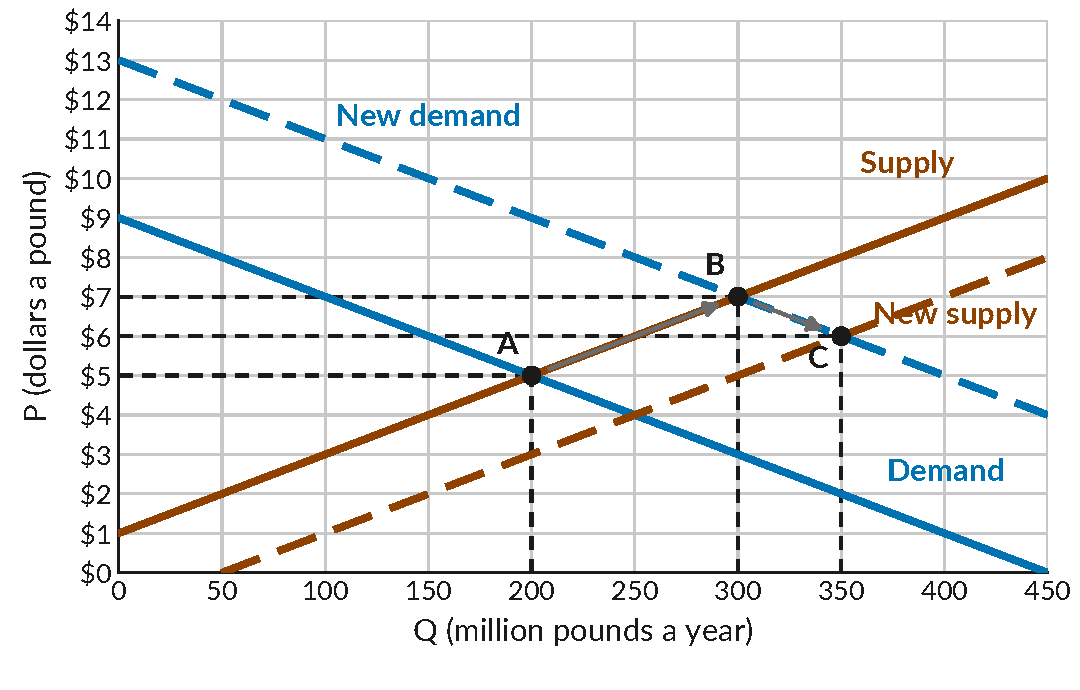
\includegraphics[width=0.74\linewidth, alt={Dollars a pound from 0 to 14 on the vertical axis with gridlines every dollar, and million pounds a year from 0 to 450 on the horizontal with gridlines every 50. Demand falls from 9 dollars at zero. A dashed new demand line runs parallel to it, 200 million pounds further right. Supply rises from 1 dollar at zero, and a dashed new supply line runs parallel to it, 100 million pounds further right. A marks 200 million pounds at 5 dollars where demand meets supply. B marks 300 at 7 dollars where new demand meets supply. C marks 350 at 6 dollars where new demand meets new supply. Dashed guides run from each point to both axes, and small arrows run along supply from A to B and along new demand from B to C.}]{figures/quinoa-key.pdf}
\else
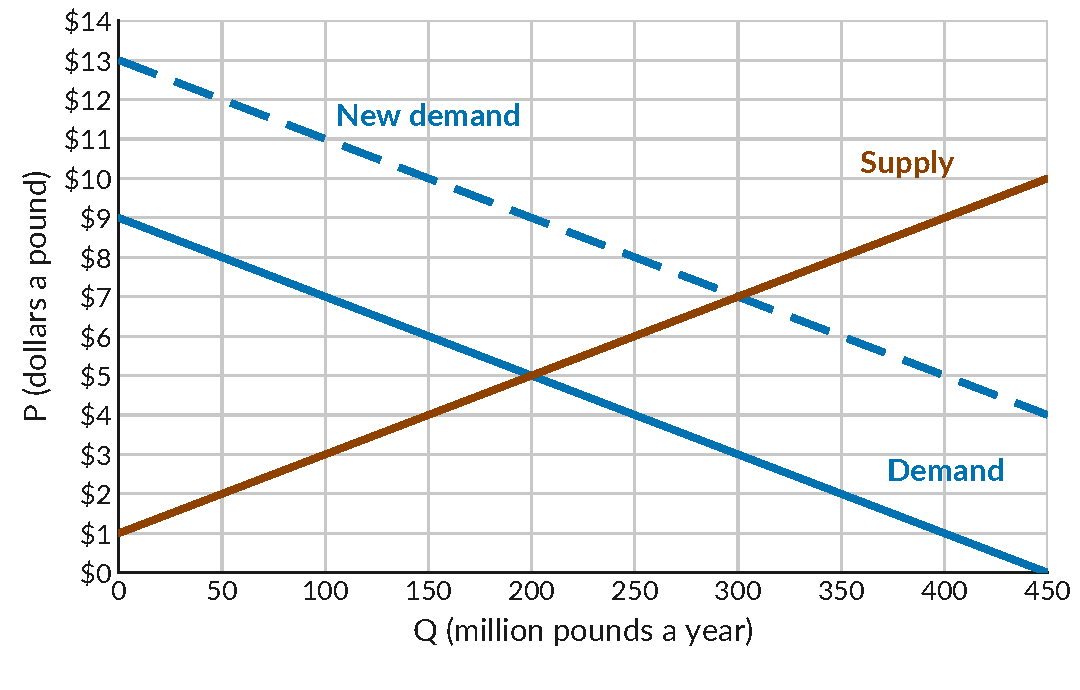
\includegraphics[width=0.74\linewidth, alt={A plotting grid, dollars a pound from 0 to 14 on the vertical axis with gridlines every dollar, and million pounds a year from 0 to 450 on the horizontal with gridlines every 50. Demand falls in a straight line from 9 dollars at zero. A dashed line labelled New demand runs parallel to it, 200 million pounds further right, starting from 13 dollars. Supply rises in a straight line from 1 dollar at zero.}]{figures/quinoa.pdf}
\fi
\end{center}

\qpart{a}{1} What are the equilibrium price and quantity before the boom? Mark this point, $A$, on the graph.
\work{1.5}
\sol{\$5 and 200 million pounds, where demand crosses supply. At that price buyers want exactly what farmers offer.}

\qpart{b}{1} After the boom, at the old price, how much do buyers want and how much do farmers offer? Is there excess demand or excess supply, and how much?
\work{2}
\sol{At \$5, buyers now want 400 and farmers still offer 200. That is an excess demand of 200 million pounds: some buyers go without.}

\qpart{c}{1} What are the new equilibrium price and quantity? Mark this point, $B$, on the graph.
\work{1.5}
\sol{\$7 and 300 million pounds, where new demand crosses supply.}

\ifsolutions\else\clearpage\fi
\qpart{d}{1.5} No one announces the new equilibrium price. Explain how the price gets from \$5 to the new equilibrium.
\ifsolutions\else\vspace{\stretch{3}}\fi
\sol{At \$5 buyers want more quinoa than farmers have, so some go without, and sellers see that they could charge more. As the price rises, farmers supply more, since pounds that cost more to grow are now worth growing, and some buyers buy less. This goes on until buyers want exactly what farmers offer, at \$7.}

\qpart{e}{1.5} In the move from $A$ to $B$, did the supply curve shift? What happened to the quantity supplied, and why?
\ifsolutions\else\vspace{\stretch{3}}\fi
\sol{No. Farmers' costs have not changed, so at any given price they would offer the same amount as before. They supply more, 300 rather than 200, only because the higher price makes it worth growing pounds that cost more.}

\ifsolutions\else
\begin{center}
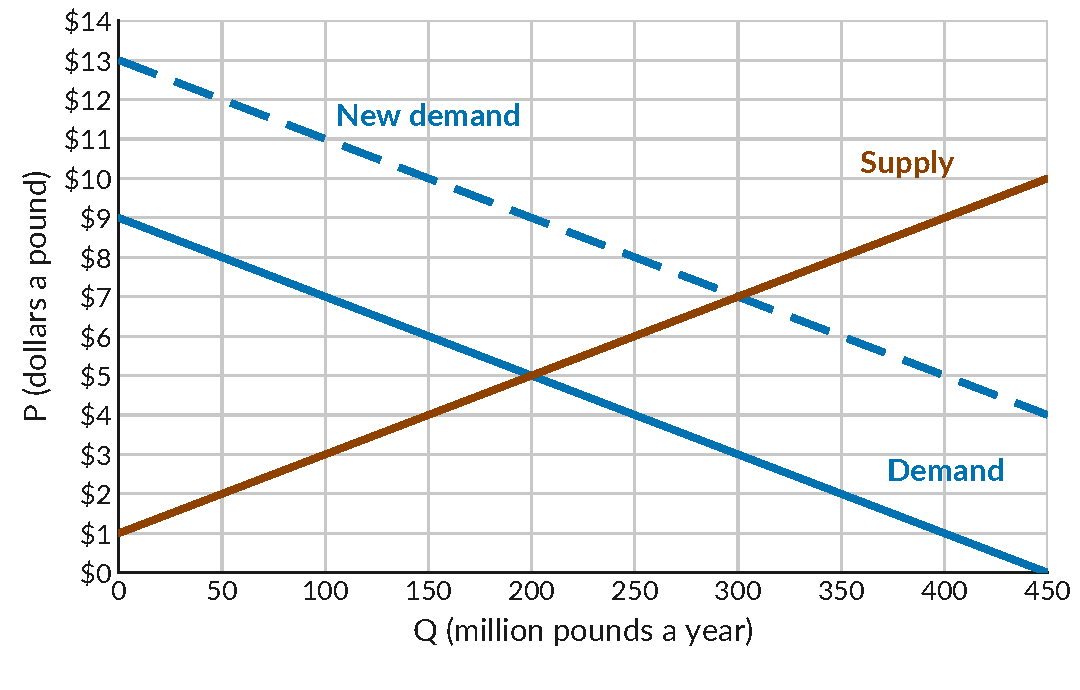
\includegraphics[width=4.5in, alt={A plotting grid, dollars a pound from 0 to 14 on the vertical axis with gridlines every dollar, and million pounds a year from 0 to 450 on the horizontal with gridlines every 50. Demand falls in a straight line from 9 dollars at zero. A dashed line labelled New demand runs parallel to it, 200 million pounds further right, starting from 13 dollars. Supply rises in a straight line from 1 dollar at zero. The same graph as on the front of this sheet, for the parts below.}]{figures/quinoa.pdf}
\end{center}
\fi

\qpart{f}{1} In the following years, the high price draws more land and more farmers into quinoa, who offer 100 million pounds more at every price. Draw the new supply curve on the graph above.
\ifsolutions\else\vspace{\stretch{1}}\fi
\sol{See the plot above: the dashed line is parallel to supply and 100 further right.}

\qpart{g}{1} At \$7, how much would farmers now offer, and how much do buyers want? Is there excess demand or excess supply, and how much?
\ifsolutions\else\vspace{\stretch{2}}\fi
\sol{Farmers would now offer 400, and buyers want 300. That is an excess supply of 100 million pounds: farmers are left with quinoa they cannot sell, so they cut their prices.}

\qpart{h}{1} What are the new equilibrium price and quantity? Mark this point, $C$, on the graph.
\ifsolutions\else\vspace{\stretch{1}}\fi
\sol{\$6 and 350 million pounds, where new demand crosses new supply.}

\qpart{i}{1} So in response to the boom, what does the price do over time, and why?
\ifsolutions\else\vspace{\stretch{2}}\fi
\sol{At first the price jumps, from \$5 to \$7, since the same farmers can only grow more at a higher cost. The high price makes quinoa profitable, so over the following years new land and farmers come in, and that extra supply brings the price back down. It settles at \$6, below the first jump, with more quinoa sold than ever.}
